\documentclass[main.tex]{subfile}
\begin{document}
\section{Test}
\subsection{Linux Kernel Modules}
Vi har kun udført en test af vores kerne modul. Denne test bygger på hvorvidt modulete kan installeres og afinstalleres. I samme forbindelse testes der også at modulet er i stand til at skrive til kernens buffer. Figur \ref{fig:part1_dmesg} viser udskrift i terminalen af beskeder gemt i kernens buffer fra indstættelse til fjernelse af modulet.
\begin{figure}[H]
\center
\fbox{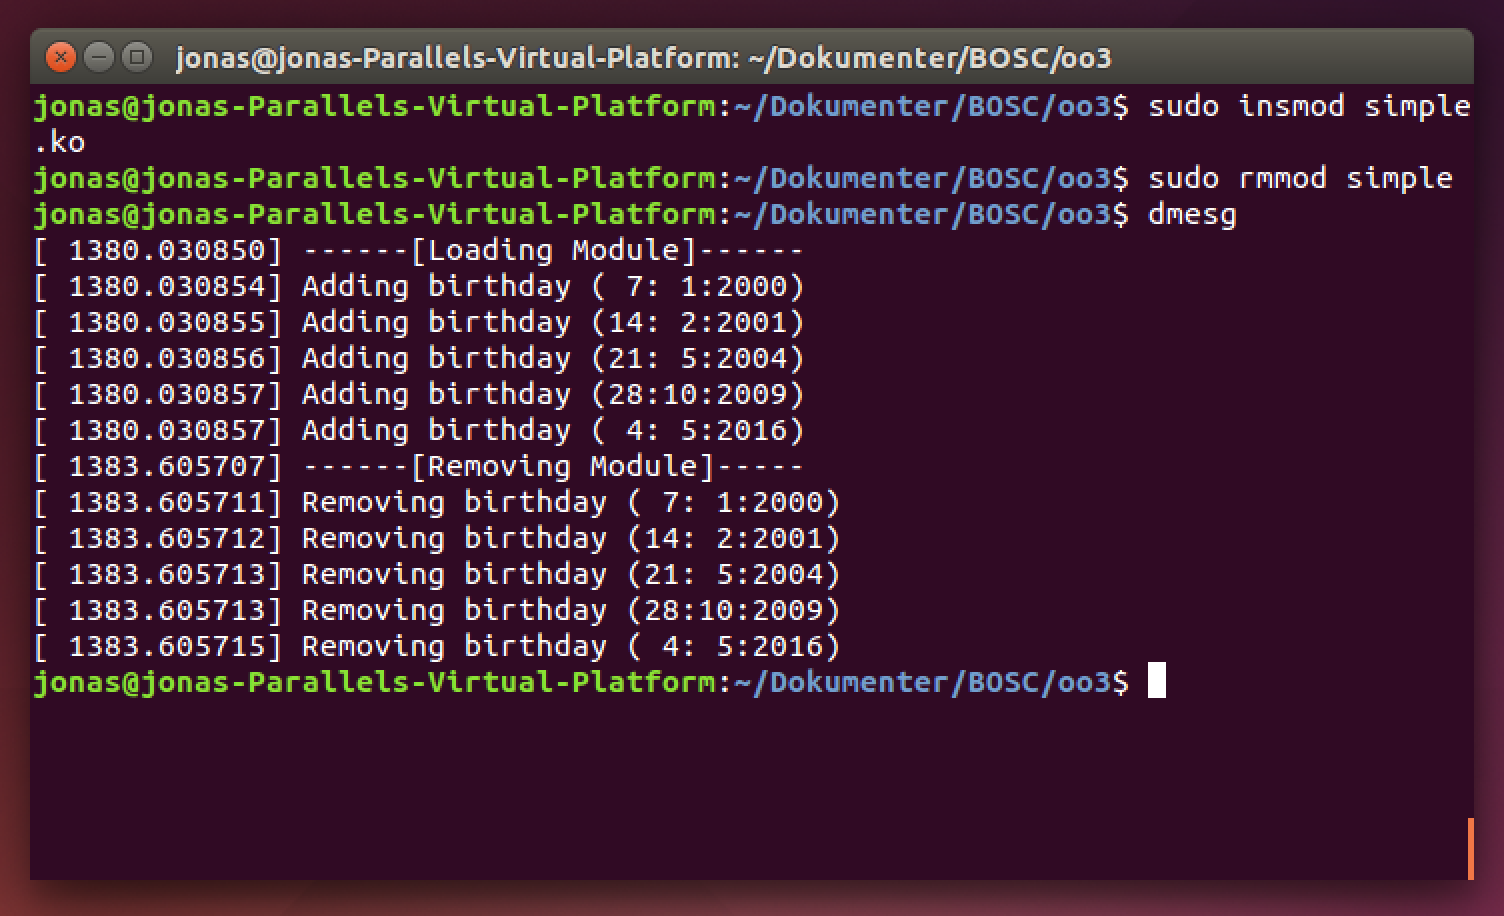
\includegraphics[width=0.95\textwidth]{part1_dmesg.png}}
\caption{Print af kernens buffer til terminalen.}
\label{fig:part1_dmesg}
\end{figure}

\subsection{Linux Kernel Module for Listing Tasks}
Silberschatz foreslår at man afprøver sin løsning ved i kommandolinien at kalde \texttt{ps -el} og \texttt{ps -eLf}. Disse systemkald returnerer hhv. alle nuværende tasks og alle nuværende tasks plus barneprocesser. Derudover skriver han også at tasks er dynamiske, og listerne kan afvige fra vore egne udskrift. Ved at køre de to systemkald får vi dog resultater som umiddelbart lader til at stemme overens med de resultater vores løsning giver.\\

Udover denne metode har vi implementeret en ganske simpel tæller, som i løbet af iterationen summerer hvor mange aktive processer der observeres, og udskriver resultatet til loggen. Resultatet af disse summeringer har ligget omkring 157 for tasks alene og 531 på samtlige processer. Linierne med summeringskoden er udkommenteret i afleveringen.\\

\begin{figure}[H]
\center
\fbox{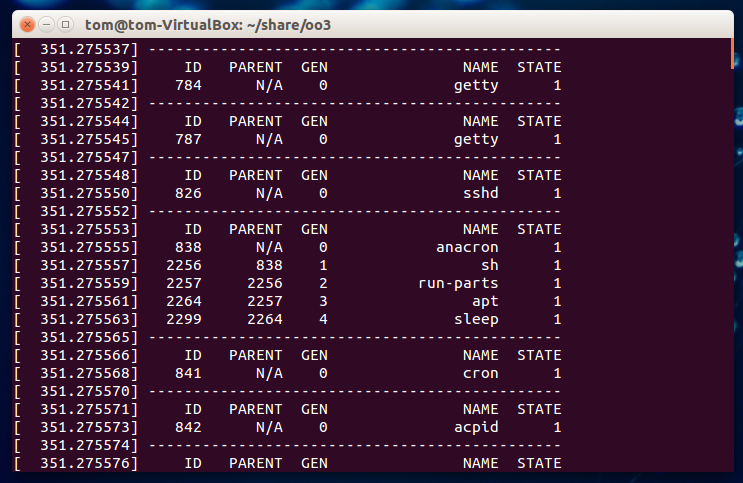
\includegraphics[width=0.95\textwidth]{part2_dmesg.png}}
\caption{Tasks og barneprocesser printet til kernel buffer loggen.}
\label{fig:part1_dmesg}
\end{figure}

Til sidst har vi udvidet den printede information til at indeholde en proces’ forældres ID nummer, samt processens generations nummer. Dette betyder, at det er muligt for en given ‘procesfamilie’ at kontrollere i hvilken rækkefølge processerne har avlet hinanden, og se at de enkelte processer skrives ud i den påkrævede orden.
\end{document}